\documentclass[SDSUThesis.tex]{subfiles} 
\begin{document}

\newpage

%% numbers following sections with A, B, C..
\appendix
\label{appendix}
\begin{center}
APPENDIX\\
\end{center}
\addcontentsline{toc}{section}{APPENDIX}

%%\section{Example Graphics} 

%%\begin{figure}[h!]
%%\scriptsize
%%$$
%%\begin{array}{cc}
%%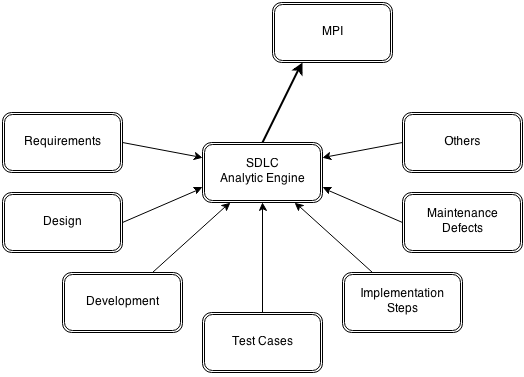
\includegraphics[width=0.2\textwidth]{sdlc-ae.png} &
%%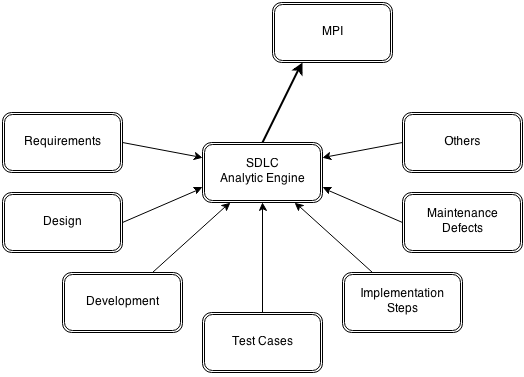
\includegraphics[width=0.2\textwidth]{sdlc-ae.png}\\
%%(a) & (b) \\
%%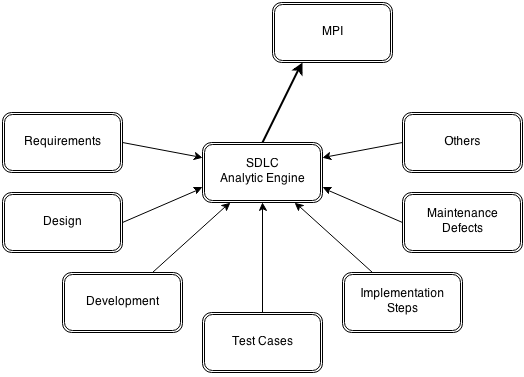
\includegraphics[width=0.2\textwidth]{sdlc-ae.png} &
%%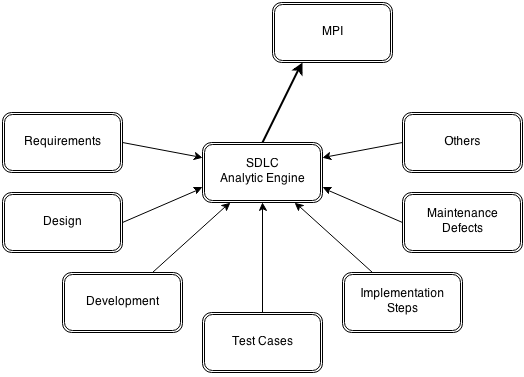
\includegraphics[width=0.2\textwidth]{sdlc-ae.png}\\
%%(c) & (d) \\
%%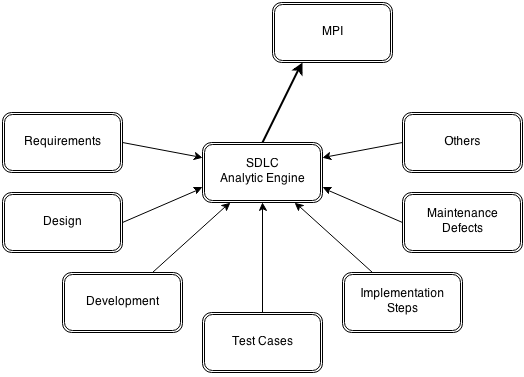
\includegraphics[width=0.2\textwidth]{sdlc-ae.png} &
%%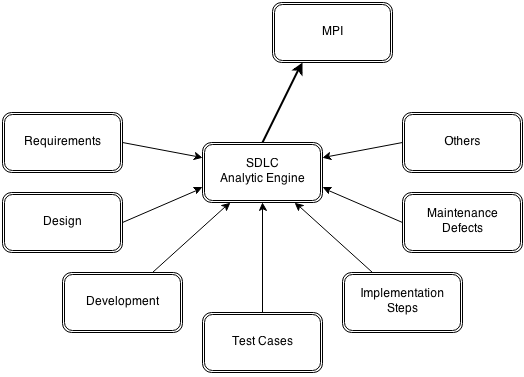
\includegraphics[width=0.2\textwidth]{sdlc-ae.png}\\
%%(e) & (f) \\
%%\end{array}
%%$$
%%\caption{A graphic in the appendix}
%%\end{figure}

%% Prints all figures and tables on the page and begins a new page
%% http://www.astro.rug.nl/~kuijken/latex.html
%%\clearpage

\section{CASE STUDY SOURCE CODE} 
\label{app:case}

\subsection{R CODE - QUALITY} 
\scriptsize{
\begin{lstlisting}[language=R]
# Load the Quality data.
setAs("character","myDate", function(from) as.Date(from, format="%m/%d/%Y") )
setClass('myDate')

quality_data <- read.csv('quality_data_clean.csv', 
        colClasses=c('factor','myDate','myDate','numeric','numeric',
        'numeric','numeric','numeric','numeric','numeric') )
str(quality_data)
head(quality_data)
summary(quality_data)

# Get data prior to 2013
old_quality_data = quality_data[quality_data$MONTH_DT <= as.Date('2013-12-31') ,]
str(old_quality_data)
pairs(old_quality_data[,c('TOTAL_TIX','EST_DEV_RES_HRS')] )

# Separate out large (>1000 hours) and small projects
large_quality_data = old_quality_data[old_quality_data$EST_DEV_RES_HRS >= 1000,]
str(large_quality_data)
largefit <- lm(TOTAL_TIX ~ EST_DEV_RES_HRS + DFTS_CNT_SIT + DFTS_CNT_UAT , 
        data=large_quality_data)
summary(largefit)
largefit_sigma = summary(largefit)$sigma
pairs(large_quality_data[,c('EST_DEV_RES_HRS','DFTS_CNT_SIT',
        'DFTS_CNT_UAT','TOTAL_TIX')])

small_quality_data = 
        old_quality_data[old_quality_data$EST_DEV_RES_HRS < 1000 
            && old_quality_data$APP != 'App 86' ,]
str(small_quality_data)
smallfit <- lm(TOTAL_TIX ~ EST_DEV_RES_HRS + DFTS_CNT_SIT + DFTS_CNT_UAT , 
        data=small_quality_data)
summary(smallfit)
smallfit_sigma = summary(smallfit)$sigma
pairs(small_quality_data[,c('EST_DEV_RES_HRS','DFTS_CNT_SIT',
        'DFTS_CNT_UAT','TOTAL_TIX')])

# predict new data  
new_large_quality_data = 
        quality_data[quality_data$MONTH_DT > as.Date('2013-12-31') 
            & quality_data$MONTH_DT < as.Date('2014-12-31') 
            & quality_data$EST_DEV_RES_HRS >= 1000,]
new_small_quality_data = 
        quality_data[quality_data$MONTH_DT > as.Date('2013-12-31') 
        & quality_data$MONTH_DT < as.Date('2014-12-31') 
        & quality_data$EST_DEV_RES_HRS < 1000,]
new_large_quality_data$PREDICTION = 
        predict(largefit, newdata=new_large_quality_data)
new_large_quality_data$SCORE = 
        (new_large_quality_data$PREDICTION - new_large_quality_data$TOTAL_TIX)
        / (6 * summary(largefit)$sigma)
new_large_quality_data[,c('APP','MONTH_DT','TOTAL_TIX','PREDICTION', 'SCORE')]

new_small_quality_data$PREDICTION = predict(smallfit, newdata=new_small_quality_data)
new_small_quality_data$SCORE = 
        (new_small_quality_data$PREDICTION - new_small_quality_data$TOTAL_TIX)
        / (6 * summary(smallfit)$sigma)
new_small_quality_data[,c('APP','MONTH_DT','TOTAL_TIX','PREDICTION', 'SCORE')]

#Combine new data  
new_quality_data = rbind(new_large_quality_data, new_small_quality_data)
str(new_quality_data)
summary(new_quality_data)
  
aggregate(SCORE ~ MONTH_DT, new_quality_data, mean)

# TODO include
# numerical summary stats, graphical summaries,
# dist of variables(hist used for guidance), associations among variables
\end{lstlisting}}

\subsection{}

\end{document}